\documentclass[UKenglish]{beamer}

\usetheme{Madrid}

% Localisation
\usepackage{babel}
\usepackage{csquotes}
\usepackage[useregional]{datetime2}

% Tables
\usepackage{caption} % Pacify ctable caption warnings.
\usepackage{ctable}

% Images
\usepackage{graphicx}
\graphicspath{{img/}}

%%% Title page

\title[CS7IS2 Project Presentation]%
{Rubik's Cube: Artificially Intelligent Solvers}

\author[O'Sullivan, William]{
  W.~O'Sullivan\inst{1}     \and
  B.~Contovounesios\inst{2} \and
  T.~Ijaz\inst{3}           \and
  F.~\'O Suibhne\inst{1}}

\institute[TCD]{
  \inst{1}%
  High Performance Computing MSc\\
  School of Maths
  \and
  \inst{2}%
  Integrated Computer Science BA \& MCS\\
  School of Computer Science \& Statistics
  \and
  \inst{3}%
  Computer Science: Intelligent Systems MSc\\
  School of Computer Science \& Statistics
}

% Replace title page date with institution; keep date in footer.
\date[\DTMdisplaydate{2021}{04}{27}{-1}]{Trinity College Dublin}

\begin{document}

\frame{\titlepage}

\begin{frame}
  \frametitle{The Rubik's Cube}
  \begin{itemize}
  \item A Rubik's Cube is a $3\times 3\times 3$ set of 26 ``cubies'', the small constituent cubes on the face of the object. The cubies can pivot about the centre of the cube, and the faces can be manipulated by rotation.
  \end{itemize}

  \begin{figure}
    \centering
    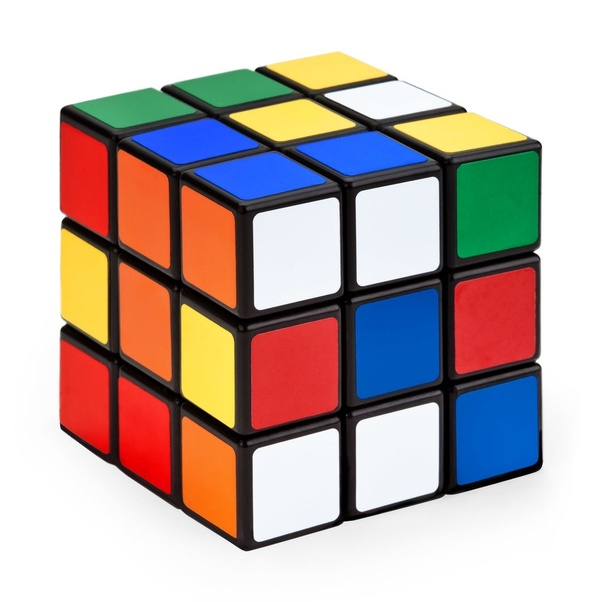
\includegraphics[width=0.35\linewidth]{scrambled-cube}
    \caption{A timeless classic!}
  \end{figure}
\end{frame}

\begin{frame}
  \frametitle{The Rubik's Cube}
  \begin{itemize}
  \item The Rubik's Cube remains a popular puzzle to this day, and whilst the cube has been solved analytically, it still serves as a fascinating problem for those of us concerned with how artificially intelligent agents solve problems.
  \item Our research has specifically examined methods for solving Rubik's Cubes (and its simpler $2\times 2\times 2$ sibling the Pocket Cube) that do not rely on human knowledge. That means that we only establish the conditions of the state space and cost functions for the respective techniques, but we do not avail of analytical solutions to the cube.
  \end{itemize}
\end{frame}

\begin{frame}
  \frametitle{Deep Reinforcement Learning w/ A$^\ast$ Search}
  \begin{itemize}
  \item Reinforcement Learning (RL) involves exploring state spaces in order to determine optimal policies for maximising rewards. Deep Reinforcement Learning (DRL) leverages Deep Learning to handle very large state spaces by training models to more efficiently approximate domain functions.
  \item Whilst DRL certainly reduces the number of states that an agent has to explore (the Rubik's Cube contains $ > 10^{19}$ unique states, and only one solution state), the sparsity of the state space means reaching the goal state must be in some way guaranteed.
  \item Autodidactic Iteration is the process whereby a solved cube is scrambled, the according moves recorded, and the move list and scrambled state are used as an input for the DRL training. This ensures that the goal state can always be reached, ultimately resulting in the solver learning how to design policies which solve the cube faster.
  \end{itemize}
\end{frame}

\begin{frame}
  \frametitle{Deep Reinforcement Learning w/ A$^\ast$ Search}
  \begin{itemize}
  \item The actual solution of the cube is then performed using a weighted A$^\ast$ Search, using the trained model as a heuristic for the distance of a given state from the goal state.
  \item At each node, the successors are examined to see which node presents the lowest total cost according to both the cost from the starting node and the cost given by the heuristic.
  \item This corresponds to building out a policy of the fewest moves, with different weightings determining whether approximate solutions are prioritised earlier or whether much closer solutions are favoured albeit further down the line.
  \end{itemize}
\end{frame}

\begin{frame}
  \frametitle{Genetic Algorithms}
  \begin{itemize}
  \item Genetic Algorithms (GA) work on a process that mimics Natural Selection, whereby individuals (that together create a population) represent approximate solutions. Over generations, through reproduction, mutation or simply being ``well-suited'', individuals are able to pass along their characteristics.
  \end{itemize}

  \begin{figure}
    \centering
    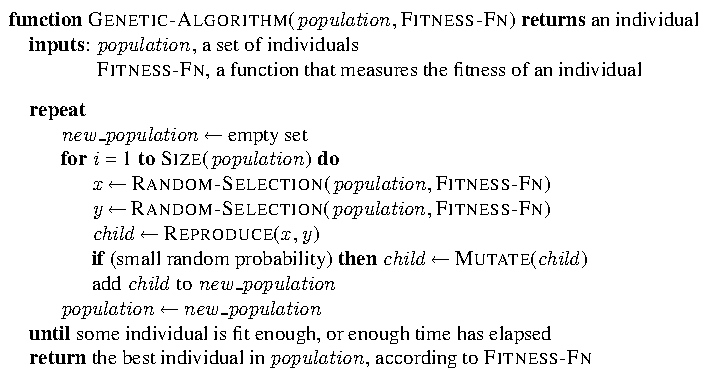
\includegraphics[width=0.75\linewidth]{genetic-algorithm}
    % \caption{Over several generations an individual that best satisfies the fitness criteria emerges. In our case, that means minimising a cost function.}
  \end{figure}
\end{frame}

\begin{frame}
  \frametitle{Genetic Algorithms}
  \begin{itemize}
  \item Reproduction accounts for 60\% of the population. Individuals with a good fitness have a higher chance of reproducing, and this entails two parents coming together and each having half of their characteristics go on to form a new individual. In the context of solving Rubik's Cubes, this means mixing together their moves to form a new policy.
  \item Mutation accounts for 30\% of the population whereby an individual can undergo a change in a small number of the moves in their policy, and in random locations.
  \item Finally, 10\% of the population who are of the highest fitness persist into the next generation, to give them an additional chance to pass along their satisfactory characteristics.
  \end{itemize}
\end{frame}

\begin{frame}
  \frametitle{Simulated Annealing}
  \begin{itemize}
  \item Simulated Annealing (SA) is an approach that combines a stochastic method with an iterative improvement algorithm. By moving from a higher randomness state to a lower randomness state over time, the algorithm converges to produce a solved cube.
  \end{itemize}

  \begin{figure}
    \centering
    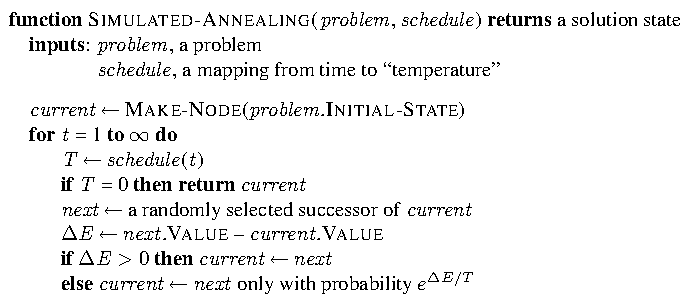
\includegraphics[width=0.75\linewidth]{simulated-annealing}
    % \caption{Over several generations an individual that best satisfies the fitness criteria emerges. In our case, that means minimising a cost function.}
  \end{figure}
\end{frame}

\begin{frame}
  \frametitle{Simulated Annealing}
  \begin{itemize}
  \item SA is an approach originally designed to model (you guessed it) annealing, whereby a material, typically a metal, is heated to relieve stress. It is then cooled gradually to allow new structures to form such that the ductility is increased---a preferable configuration.
  \item It is in this way that we treat the Rubik's Cube solver, whereby we start with a ``high-temperature'' system and as the system cools according to a specified cooling rate, configurations of moves which minimise the cost-function arise.
  \item If the system does not converge, it undergoes a reheating, whereby the cooling resumes from a temperature slightly above the end temperature. This cooling and reheating allows for the last few degenerate states to resolve and achieve a true global minimisation of the cost function.
  \end{itemize}
\end{frame}

\begin{frame}[b]
  \frametitle{Findings}
  \begin{itemize}
  \only<1>{\item The various methods were compared using the runtime and the number of moves required to reach a solution.}
  \only<2>{\item In this table we can readily observe that DRL + A$^\ast$ consistently beat the baseline using domain knowledge---a very impressive feat.}
  \only<2>{\item It consistently produced the most efficient set of moves across all of the methods, and it only lost the the SA in terms of runtime for $n=2$.}
  \only<3>{\item GA solved the $n=2$ consistently, and only solved the $n=3$ cubes 27\% of the time.}
  \only<3>{\item The difficulty was attributed to becoming stuck in the degenerate states, which were inherently difficult to select out between generations.}
  \only<4>{\item SA solved all of the cubes it was presented with, though at a prohibitively high move count.}
  \only<4>{\item This behaviour was anticipated however, as SA was the most stochastic method employed. Many unfavourable moves were selected probabilistically, leading to the bloated move count.}
  \end{itemize}

  \vfill
  \ctable{@{\extracolsep{1em}}ll*{4}{r}}{}{                       \FL
    Size  & Metric      & DRL + A$^\ast$ &  GA &    SA & Baseline \ML
    $n=2$ & Runtime (s) &            3.2 &   7 &   2.9 &       10 \NN
          & \# of Moves &             10 &  29 &  1270 &       17 \ML
    $n=3$ & Runtime (s) &           13.6 & 255 &   204 &       15 \NN
          & \# of Moves &             22 & 350 & 43623 &       32 \LL
  }
  \vspace{2em}
\end{frame}

\begin{frame}
  \frametitle{Conclusion}
  \begin{itemize}
  \item All three approaches resulted in solved $n=2$ and $n=3$ cubes without human knowledge.
  \item Of the three, Deep Reinforcement Learning combined with an A$^\ast$ Search proved most consistently optimal.
  \item That said, this investigation served as proof of concept for the possibility of Genetic Algorithms and Simulated Annealing solving $n=2$ and $n=3$ cubes without domain knowledge---approaches that had not before been present in the literature.
  \end{itemize}
\end{frame}

\end{document}
